\documentclass{beamer}
\usepackage{graphicx}
\graphicspath{ {images/} }
\usepackage[utf8]{inputenc}
\usetheme{Madrid}
\usecolortheme{default}
\mode<presentation>

%Details
\title[Simulated Annealing]{Solving Travelling Salesman Problem using Simulated Annealing}
\author[Anshuman]{Anshuman Kumar}
\institute[IIT Bombay]{
    Department of Aerospace Engineering \\
    IIT Bombay
}
\date{\today}

%Title Page
\begin{document}

\begin{frame}
    \titlepage
\end{frame}


\begin{frame}
    \frametitle{Outline}
    \tableofcontents
\end{frame}

\section{Travelling Salesman Problem}
\begin{frame}
    \frametitle{Travelling Salesman Problem}
    \begin{definition}
        A \alert{Travelling Salesman Problem} asks the following
        question: Given a list of cities and the distances between each
        pair of cities, what is the shortest possible route that visits
        each city exactly once and returns to the origin city?
    \end{definition}
\end{frame}

\begin{frame}
    \frametitle{Simple Travelling Salesman Problem with 20 cities}
    \begin{figure}[t]
        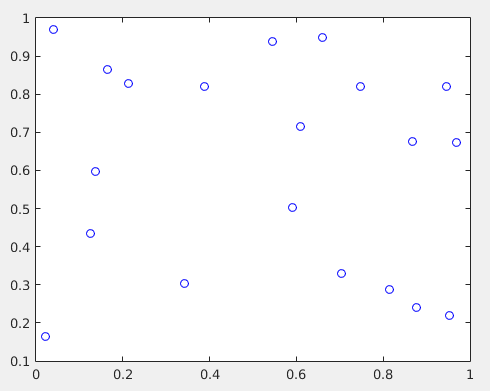
\includegraphics[width = 8cm]{20cities}
        \caption{Showing 20 cities at different position}
        \centering
    \end{figure}
\end{frame}

\section{Simulated Annealing}

\begin{frame}
    \frametitle{Simulated Annealing}
    \begin{definition}
        Simulated annealing (SA) is a generic probabilistic metaheuristic
        for the global optimization problem of locating a good 
        approximation to the global optimum of a given function in a
        large search space. It is often used when the search space is
        discrete (e.g., all tours that visit a given set of cities).
    \end{definition}
\end{frame}

\section{Problem Model}
\begin{frame}
    \frametitle{Modelling of Problem}
    \begin{block}{Objective}
        Minimise the total distance travelled by Salesman \\
    \end{block}
    Randomly index the cities as 1,2,3,4 .... n
    \begin{figure}[t]
        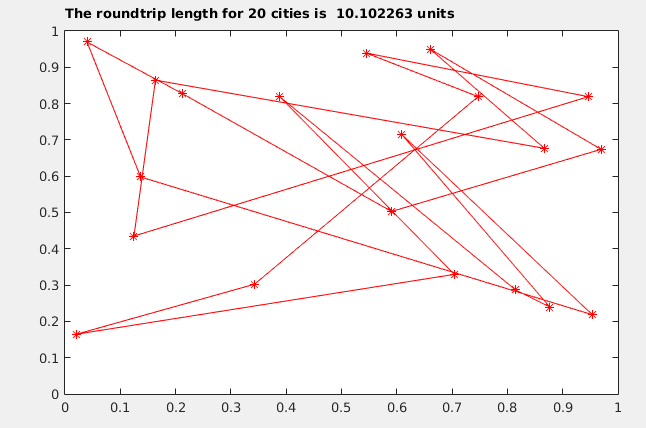
\includegraphics[width = 6cm]{randomcities}
        \caption{Showing 20 cities with travel route}
        \centering
    \end{figure}
\end{frame}

\begin{frame}
    \frametitle{Distance function and Swaps}
    Calculate Distance
    \begin{itemize}
        \item Recursively add distance from i to i+1 starting from 
            1, and go till n-1.
        \item Then add the distance of n from 1;
    \end{itemize}
    \begin{block}{Swap}
        Swapping is just changing the index of cities\\
        Example \alert{temp = 5, 5 = 20 , 20 = temp}
    \end{block}
\end{frame}

\begin{frame}
    \frametitle{Iteration}
    \begin{itemize}
        \item Calculate the distance.
        \item Based on temperature decide the numbers of Swaps.
        \item Produce a new city list based on random swaps.
        \item Calculate the distance again.
        \item If distance is less than old distance make your new city list as current list.
        \item If distace is more based on probablity decide which city list to choose.
    \end{itemize}
\end{frame}

\section{Conclusions}
\begin{frame}
    \frametitle{Optimised path for Salesman}
     \begin{figure}[t]
        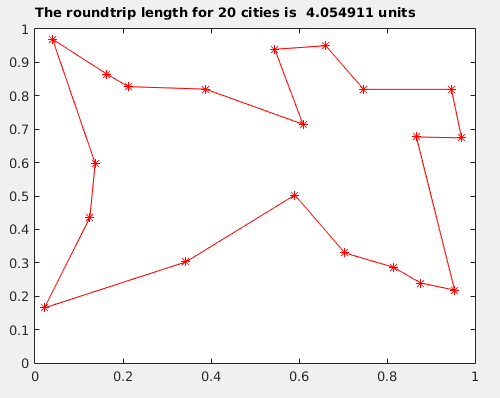
\includegraphics[width = 8cm]{optimisedcity}
        \caption{Showing 20 cities with optimised travel route}
        \centering
    \end{figure}
\end{frame}

\begin{frame}
    \frametitle{Conclusions}
    \begin{itemize}
        \item Most of the time results are exactly same as the real answer.
        \item Sometime we did't get the exact solution, but the answer is too near to real solution.
        \item This algorithm takes much less time than brute force method.
    \end{itemize}
\end{frame}
\end{document}

